La iniciativa de la Web Semántica puede ser divergente en sus enfoques para los
diferentes escenarios de aplicación, pero lo que está perfectamente definido
es su apoyo en el uso de \textbf{ontologías}~\cite{Sowa99knowledge}. 

\subsubsection{Ontologías en la Web Semántica}
La evolución de la web a través de la Web Semántica, proporciona un nuevo
espacio de publicación de recursos (documentos) que junto con las nuevas tecnologías de
la información generan un entorno con unas condiciones inigualables para la
divulgación de contenido.

Uno de los principales problemas de la web actual es la inmensa cantidad de
información que se publica obviando cualquier procedimiento de control, creando
grandes bases de datos, recursos y conocimiento, cuya explotación no es eficiente, ya que
en muchos casos sólo está preparada para ser procesada o bien por agentes
humanos o por agentes \textit{software}.

Las ontologías se presentan como una forma para la organización de conocimiento
y contenido heterogéneo en el ámbito de la Web Semántica, estableciendo un enlace entre el procesamiento humano de recursos y el
automático, realizado entre agentes \textit{software}. Paralelamente, las ontologías se utilizan como
instrumentos para la desambiguación del lenguaje natural. Constituyendo en definitiva un mecanismo para 
la realización de la comunicación entre agentes de forma eficiente
basándose en un conocimiento común y compartido. En la Sección~\ref{ontologias} se describen más amplia y genéricamente los modelos de conocimiento basados en ontologías.

\subsubsection{Arquitectura para la Web Semántica}\label{sect:arch-ws}
En un primer momento, la arquitectura para la Web Semántica, más conocida como
``tarta o pila de la Web Semántica'', ver Figura~\ref{fig:stack-2002}, se diseño con diferentes capas de abstracción, 
construyen un \textit{framework} semántico, recogiendo supuestamente, todas las necesidades para la gestión del
conocimiento. Cada una de las capas enriquece a la inmediatamente inferior
proveyendo nuevos servicios o niveles de formalización superior del conocimiento.

\begin{figure}[!htbp]
\centering
	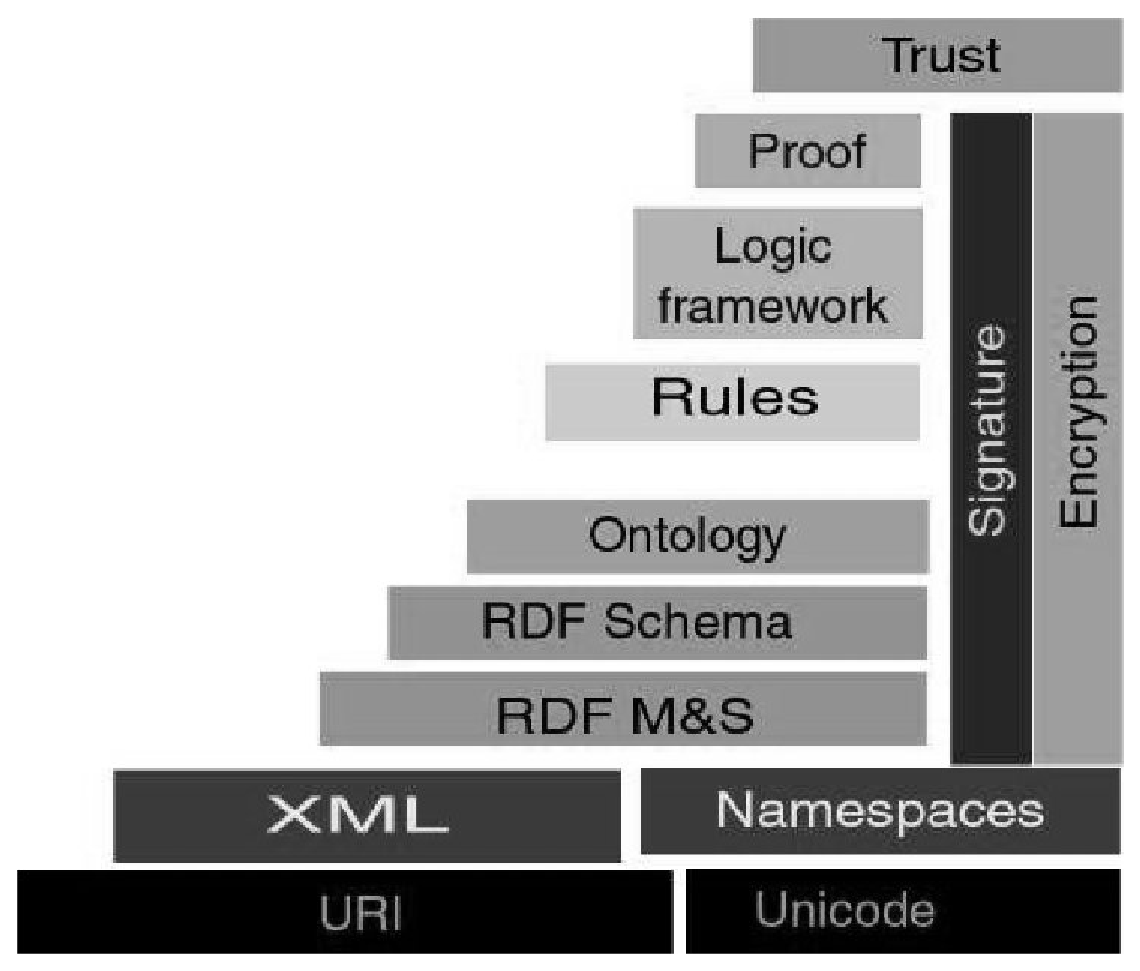
\includegraphics[width=10cm]{images/sw-stack-2002}
\caption{Arquitectura Web Semántica 2002.}
\label{fig:stack-2002}
\end{figure}

A continuación se explica someramente la intención de cada una de las capas y el por qué
de su presencia:
\begin{description}
\item[\gls{URI}/\gls{IRI}-Unicode.] Para dar un soporte estándar a una tecnología existen
dos factores fundamentales: nombrado e identificación única de cada uno de los
recursos y codificación de los mismos. Por esta doble razón aparecen los \textit{Unified
Resource Identifier}y la codificación estándar Unicode, implementada principalmente en UTF-8.
\begin{example}
URI: protocolo:dirección:directorio:recurso, \url{http://www.josemalvarez.es/foaf.rdf}
\end{example}

\item[\gls{XML}~\cite{XML11}.] lenguaje extensible de marcas (\textit{eXtensible Markup
Language}) es un formato estándar creado para la estructuración de datos.
Hoy en día se encuentra regulado por el \gls{W3C} que es el encargado de realizar las distintas
especificaciones y versiones desde Febrero de 1998. XML está basado en \gls{SGML}
(\textit{Standard Generalized Markup Language}, ISO 8879) que ya había sido establecido
en 1986. El uso principal de XML es la estructuración de datos, pero en general es utilizado por todas
aquellas aplicaciones informáticas en las cuales se pueda representar la información jerárquicamente.
El lenguaje XML es en sí mismo un metalenguaje utilizado ampliamente para definir otros
lenguajes. Consta entre otros, de elementos y atributos. Su orden y jerarquía
son los encargados de formar el lenguaje que definimos con XML. No se dispone de etiquetas predefinidas, como podría ser \gls{HTML}, esto
se deja a labor del usuario que es el encargado de definir un conjunto de elementos con sus
etiquetas asociadas, la semántica de los documentos es proporcionada por la aplicación que use
esos datos. Para definir la estructura de un documento XML, es decir, una 
gramática que indique el orden de los elementos y su jerarquía, lo podemos conseguir de
dos formas utilizando: 1) \gls{DTD} o 2) \gls{XML Schema}~\cite{XMLSchema}.

Es importante resaltar que un documento bien formado no es lo mismo que un documento
válido, un documento estará bien formado cuando siga las reglas sintácticas de
formato XML, mientras que un documento será válido si todos sus elementos están en orden correcto de anidación y está bien formado. Algunas de las razones 
por las que es interesante utilizar XML son las siguientes:
\begin{itemize}
\item Estándar para el intercambio de datos.
\item Facilidad de uso.
\item Legibilidad.
\item Implantación.
\item Extensibilidad.
\item Separación entre formato y contenido.
\item Tratamiento multiplataforma.
\item Es libre, especificaciones disponibles. 
\end{itemize}

\begin{figure}[!htbp]
\centering
\lstinputlisting[language=XML]{examples/events.xml}
\caption{Ejemplo de fichero XML.}
\label{fig:ejemplo-xml}
\end{figure}

Como aplicación práctica de XML, ver Figura~\ref{fig:ejemplo-xml}, y debido a la necesidad de tratamiento
automático para diferentes fines (formatos de presentación, transformación de un
vocabulario a otro, etc.) hay que destacar \gls{XSL}~\cite{XSL} generación del
contenido a partir de un documento XML de una manera rápida, sencilla y eficaz, cuyo objetivo principal es presentar al usuario final un 
interfaz del documento más entendible con el que pueda realizar un tratamiento de la información contenida en él de una manera más
asequible, sin necesidad de conocer el formato XML.

\begin{figure}[!htbp]
\centering
	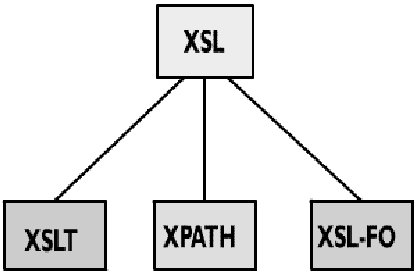
\includegraphics[width=6cm]{images/xsl}
\caption{Componentes de XSL.}
\label{fig:xsl}
\end{figure}

Por ello desde el consorcio \gls{W3C} se optó por realizar la especificación XSL con
el objetivo de presentar un modelo para el procesamiento de la información
almacenada en formato XML. La especificación redactada por el consorcio web para la transformación del contenido XML
se denomina XSL, se encarga de definir una hoja de estilo con la cual se transforma el fichero
XML en otro formato, teniendo en cuenta que la información en XML se almacena de forma
jerarquizada, con la definición de XSL se pretende poder presentar al usuario dicha información
en otros formatos estructurados como pueden ser: HTML, \gls{PDF}, etc., XSL es una especificación, pero 
el lenguaje del que hace uso para la realización de la transformación es XSLT con sintaxis de XPath~\cite{XPath}.

En \gls{XSLT} se define cómo se ha de realizar la transformación del documento XML y no
cuándo se debe realizar, la transformación del documento se realiza en distintos
pasos: 
\begin{itemize}
    \item Generación de un árbol a partir del fichero fuente de XML, esto se
    realiza mediante un procesador que analiza el documento, realizando al mismo tiempo una validación sintáctica del
mismo.
\item Procesamiento del árbol generado construyendo un nuevo árbol con la
información procesada, el recorrido del árbol generado se realiza en preorden, con la posibilidad de variar el tipo de recorrido, es importante tener en cuenta
el orden de evaluación de los nodos del árbol para así poder aplicar las
plantillas correctamente. 
\end{itemize}

El principal uso de XSLT como ha quedado patente en la introducción, es la transformación
de documentos XML para generar contenido web, lógicamente esto no aportaría demasiada potencia
a este lenguaje si solo sirviera para generar contenido web estático. En cambio usando
este lenguaje se genera contenido dinámico aplicando distintas reglas, como ejemplo se
podría obtener de una base de datos un fichero XML y con dicho fichero y una transformación
apropiada generar una página dinámica con contenidos auto-actualizables cada cierto tiempo, otro 
ejemplo de aplicación podría ser la conversión de un programa escrito en un lenguaje a otro, definiendo las reglas correctas. 
XSLT utiliza también \gls{XPath}, ver Figura~\ref{fig:xsl-example}, que es una especificación
para el acceso a los valores de los distintos nodos del árbol generados a partir del procesamiento
del fichero XML. 

\begin{figure}[!hbp]
\centering
\lstinputlisting[language=XML]{examples/events.xsl}
\caption{Ejemplo de hoja de estilo XSL.}
\label{fig:xsl-example}
\end{figure}


\item[\gls{XML Schema}~\cite{XMLSchema}.] En primer lugar es interesante diferenciar las dos
tecnologías establecidas para la definición de la estructura de un documento
XML: \begin{inparaenum}
     \item \textit{Document Type Definition} (\gls{DTD}) es un vocabulario para definir las
     reglas de construcción de un documento XML.     
     \item XML Schema: Vocabulario XML utilizado para definir otros vocabularios
     XML.  
     \end{inparaenum}

El incremento en el uso de \gls{XML} hace necesario la utilización de tecnología para poder
expresar la estructura del documento y así proceder a su validación. Aunque en principio el objetivo de ambos es el mismo: 
definir vocabularios XML para poder validarlos sintácticamente e imponer distintos tipos de 
restricciones como de cardinalidad o integridad, cada uno presenta unas características diferentes 
lo que supone que escoger entre uno u otro implique realizar un estudio de lo que se pretende desarrollar.
También disponemos de herramientas que nos permiten realizar la transformación de uno a
otro pero sólo en el sentido de DTD a XML Schema. Se puede pensar que XML Schema es el
sucesor de las DTD.

La utilización de XML Schema, ver Figura~\ref{fig:xsd-example}, se apoya en diferentes características que hacen
que su uso sea interesante en el ámbito de la Web Semántica:
\begin{itemize}
\item Espacios de nombres, permite utilizar los mismos identificadores en el
mismo documento, evitando así la ambigüedad.
\item Esquema, es la estructura que va a presentar el vocabulario XML construido, con
sus distintos elementos y atributos así como con las validaciones que sean
necesarias.
\item Documento instancia,  documento XML creado con una estructura
definida en un XML Schema y contra el cual se ``valida''.
\end{itemize}

Las razones que pueden llevar a elegir XML Schema son, entre otras, las siguientes:
\begin{itemize}
  \item Utiliza sintaxis XML.
  \item Perfectamente documentado.
  \item Define los elementos y atributos que pueden aparecer en un documento instancia.
  \item Establece la jerarquía y orden de los distintos elementos.
  \item Podemos crear distintos tipos genéricos.
  \item Extensible.
  \item Inclusión de documentos externos.
  \item Expresividad.
  \item Posibilidad de documentación.
  \item Tipos de datos simples, complejos, derivados.
  \item Expresión de restricciones de integridad y cardinalidad.
  \item Reutilización de tipos por extensión o restricción.
  \item \ldots  
\end{itemize}


\begin{figure}[!htbp]
\centering
\lstinputlisting[language=XML]{examples/events.xsd}
\caption{Ejemplo de XML Schema.}
\label{fig:xsd-example}
\end{figure}


La utilización de XML Schema es crítica en los servicios web basados en \gls{WSDL}~\cite{WSDL20} y \gls{SOAP}~\cite{SOAP11} y 
está muy asentada en entornos de desarrollo basados en Java a través de herramientas como \gls{JAXB}.

\item[\gls{RDF}~\cite{RDF}.] \textit{Resource Description Framework}, se encarga
de describir los recursos, añadiéndoles la metainformación necesaria en
un formato procesable. En la siguiente Sección~\ref{rdf} abordaremos la descripción de
RDF de manera más extensa.

\item[Ontologías:] Los documentos etiquetados constituyen una gran cantidad
de información disponible para utilizar por la máquina. Están disponibles los datos, pero
todavía no hay capacidad semántica. Es necesario construir un modelo donde ``encajar''
esos datos. Para añadir la componente semántica mediante ontologías, ver Sección
\ref{ontologias}, se pueden utilizar diferentes lenguajes, cuyo estudio se 
abordará en la Sección~\ref{lenguajes}.

\item[Capas superiores:] La arquitectura propone diferentes niveles en los
que se colocan las reglas y la lógica, debido a su complejidad todavía es precipitado definirlas por completo y las discusiones se mantienen
abiertas en grupos de trabajo del \gls{W3C} como el \gls{RIF}~\cite{rif-core}. 
Los módulos transversales de ``firma''~\cite{XML-dsig} y 
``encriptación''~\cite{XML-enc} están definidos y se
pueden encontrar como recomendaciones del W3C.

\end{description}

Aunque las ventajas de un diseño basado en capas está sobradamente demostrado en
bibliografía de ingeniería del \textit{software}, hay que resaltar que esta primera
aproximación ha sido modificada con el objetivo de recoger la realidad de la
arquitectura para la Web Semántica. Hay que tener en cuenta que la primera
versión propuesta por \textit{Tim Berners Lee} (web XML) ofrecía una visión ideal
que contemplaba todas las partes implicadas, pero que no tenía el efecto experiencia
de la construcción de aplicaciones y de los posibles problemas que se podrían
encontrar. Por ello, esta arquitectura ha sido rediseñada planteando un modelo
más cercano a la realidad, por lo menos de las aplicaciones y problemas, y que
también es conocida como las ``dos torres''~\cite{kifer05} (web RDF), ver Figura~\ref{fig:stack-2005}.

\begin{figure}[!htbp]
\centering
	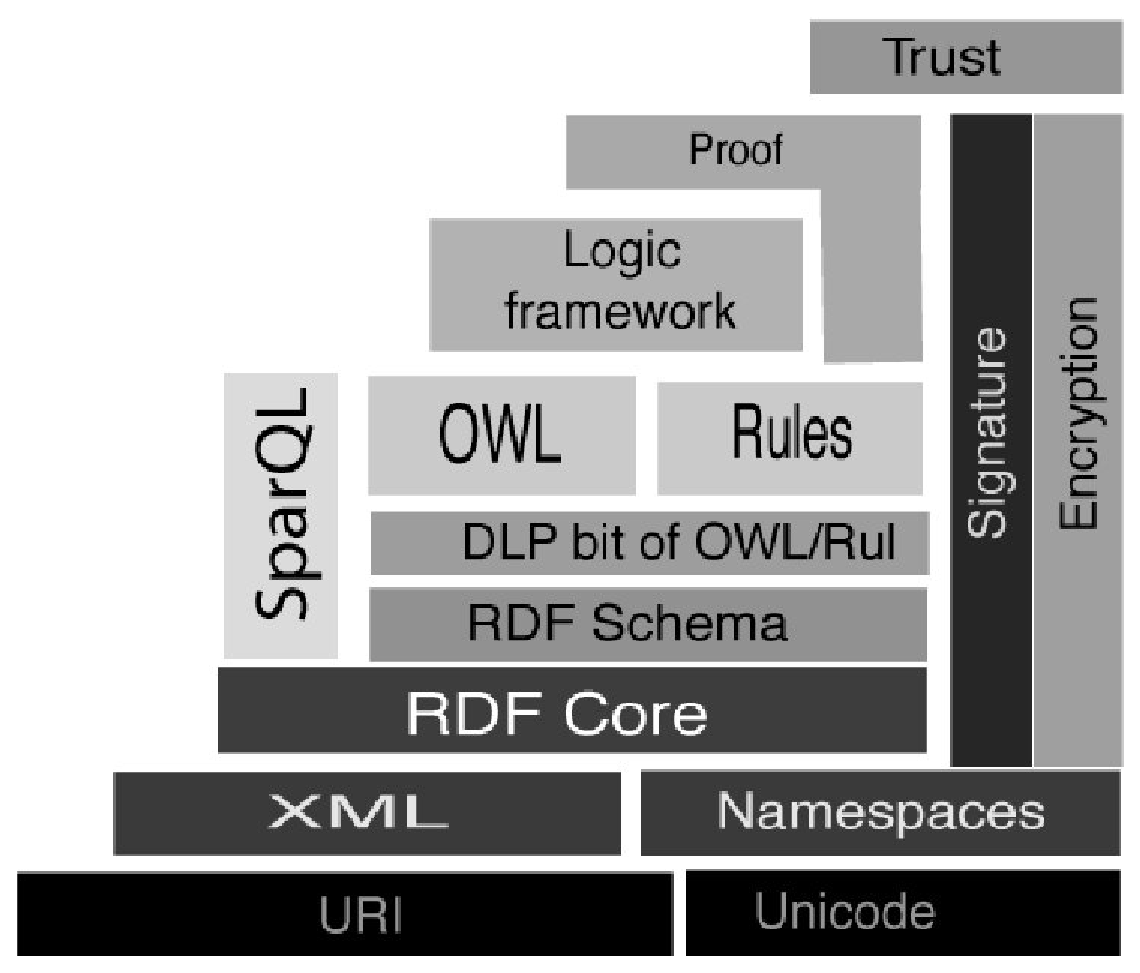
\includegraphics[width=10cm]{images/sw-stack-2005}
\caption{Arquitectura Web Semántica 2005.}
\label{fig:stack-2005}
\end{figure}

La propuesta de cambio surge porque la Lógica Descriptiva, que utiliza \gls{OWL}, no
tiene un poder expresivo suficiente para solucionar el problema de la
representación de conocimiento y razonamiento en la Web Semántica. OWL no puede
tratar con información de una forma dinámica, no tiene predicados \textit{n-arios}, no
soporta símbolos de función, etc. De ahí que se valorará la posibilidad de extender las bases
de conocimiento en OWL con reglas para aumentar la expresividad de los modelos y
ganar en capacidad de inferencia.

Las reglas, en programación lógica como PROLOG, tienen una larga tradición en
las ciencias de la computación y se llevan estudiando desde hace más de 20 años. Sin
embargo, la extensión de OWL con reglas no es una tarea sencilla. En general, las reglas 
están basadas también en un subconjunto de la lógica de primer orden, la
lógica \textit{Horn}, aunque su semántica formal es diferente, no está basada en teoría de modelos. La diferencia fundamental, aparte del tratamiento
de la negación y cuestiones de expresividad, tiene que ver con OWL, ya que, 
debido a su semántica de primer orden, utiliza la hipótesis de mundo abierto,
mientras que las reglas habituales de programación lógica utilizan mundo cerrado. 

La extensión más conocida de OWL en este sentido es \gls{SWRL}~\cite{Swrl}, que permite cláusulas
Horn como axiomas en las bases de conocimiento en OWL. Este lenguaje mantiene
el mundo abierto de OWL, pero penaliza en rendimiento debido a su alto coste computacional.

Debido a esta serie de problemas, se ha sugerido la opción de separar ontologías y
reglas (lógica descriptiva y programación lógica) y utilizar cada tecnología en casos
de uso pertinentes y apropiados. La combinación entre ambos, un objetivo verdaderamente ambicioso de la Web Semántica, 
ya no sería mediante la extensión de OWL con algún tipo de formalismo para la expresión de reglas, sino mediante la construcción
de un interfaz lógico que permita desde las reglas utilizar información definida
en las ontologías, y desde éstas, información inferida por el
comportamiento de los sistemas de reglas.

Destacar la aparición del lenguaje de consulta para RDF, \gls{SPARQL}~\cite{Sparql} y su última
versión SPARQL 1.1, creado por la necesidad de disponer de un lenguaje de acceso a los recursos
definidos en forma de grafo y con una semántica definida~\cite{Perez:2009:SCS:1567274.1567278}. El modelo semántico~\cite{citeulike:1556975} 
proporcionado por RDF permite tratar cualquier recurso como una entidad con descripción asociada. No obstante, el uso de RDF no es
suficiente para la elaboración de modelos de dominio más ricos y descriptivos, razón por la cual surge un lenguaje como OWL que apoyado sobre el modelo de RDF
permite realizar formalizaciones utilizando diferentes lógicas (principalmente \textit{Description Logics}).

\subsubsection{Lenguajes para la Web Semántica: Creando ontologías}\label{lenguajes}
La construcción de una base de conocimiento~\cite{GruberOnto} utilizando ontologías puede
realizarse con distintos lenguajes y diferentes grados de expresividad lógica~\cite{HoPa10a,Kifer:1989:FHL:66926.66939}.
La selección de la lógica apropiada para la modelización de nuestra base de
conocimiento no es una cuestión sencilla y debemos contemplar diferentes
factores: grado de computabilidad, decidibilidad, soporte razonadores, etc.
Todos ellos determinarán la lógica a utilizar ya que no se puede señalar arbitrariamente que se debe utilizar un nivel lógico cuando no es necesario para
el modelo formal.
\subsubsection{RDF}\label{rdf}
El primer lenguaje que nos encontramos para la creación de ontologías es \gls{RDF}
(\textit{Resource Description Framework}) como soporte básico a la par que potente, 
para añadir semántica a los recursos (documentos entre otros). La primera observación 
a realizar es la distinción entre: \begin{inparaenum}\item Modelo de datos, basado en
tripletas Sujeto-Predicado-Objeto. \item Formato de datos, puede utilizar RDF/XML (normativo)
como formato para la serialización del modelo.\end{inparaenum}

El modelo de datos de RDF utiliza tripletas, ver Figura~\ref{fig:rdf-model}, encargadas de describir recursos:
\begin{description}
\item[Sujeto:] recurso sobre el que vamos a realizar una afirmación. Están
identificados de forma única a través de URIs. Por ejemplo: Yo.
\item[Predicado:] es la afirmación sobre el sujeto. Por ejemplo: ``tengoNombre''.
\item[Objeto:] valor del predicado para este sujeto. Por ejemplo: ``Jose
María''@es.
\end{description}

\begin{figure}[!htbp]
\centering
	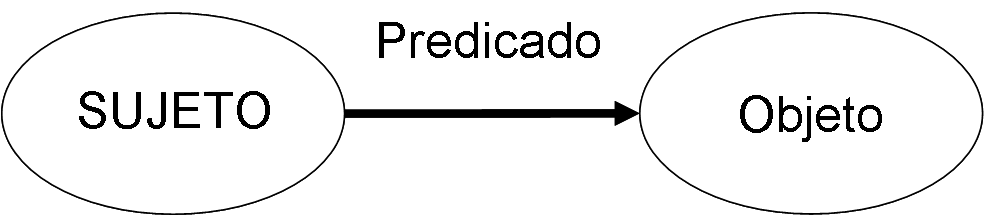
\includegraphics[width=10cm]{images/rdf-model}
\caption{Modelo de tripletas RDF.}
\label{fig:rdf-model}
\end{figure}

Usando RDF pueden realizarse afirmaciones simples sobre ``cosas'': ``Este
documento de memoria tiene de creador'' a ``Jose María Alvarez'' puede expresarse en
RDF usando la tripleta (memoria, ``tieneCreador'', ``Jose María Alvarez''). 
A su vez  se pueden generar nuevas tripletas (memoria, ``tieneFecha'',
``Enero 2012'') o (memoria, ``tieneFormato'', ``PDF''), generando así un
modelo semántico simple pero perfectamente válido. Si se le añade el uso de colecciones y 
la capacidad de ``reificación'' (afirmaciones sobre otras
afirmaciones) se conseguirá una capacidad de expresión muy potente asentada en un
sencillo lenguaje. En cuanto, a la serialización de RDF o su formato, existen diferentes estándar
perfectamente válidos para su tratamiento automático por las máquinas y más o
menos amigables para los humanos. 
\begin{itemize}
  \item \gls{RDF/XML}~\cite{rdf-syntax} formato estándar y normativo por excelencia, ver Figura~\ref{fig:rdf-n3}. 
\begin{figure}[!htbp]
\centering
  \begin{lstlisting} 
<rdf:RDF xmlns:rdf="http://www.w3.org/1999/02/22-rdf-syntax-ns#"
  xmlns:rdfs="http://www.w3.org/2000/01/rdf-schema#"
  xmlns:dc="http://purl.org/dc/elements/1.1/">
    <rdf:Description rdf:about="http://petra.euitio.uniovi.es/~i1637566/">
      <dc:creator>Jose M. Alvarez</dc:creator>
    </rdf:Description>
</rdf:RDF>  
  \end{lstlisting} 
\caption{Ejemplo de tripletas de RDF en RDF/XML.}
\label{fig:rdf-n3}
\end{figure}  

\item Otros como: \gls{RDFa}~\cite{rdfa-primer}, \gls{Turtle}~\cite{turtle-syntax}, \gls{N3}~\cite{n3-syntax} ,\gls{RDF}/\gls{JSON}~\cite{rdf-json} o RDF binario~\cite{rdf-binario}.   
\begin{figure}[!htbp]
\centering
  \begin{lstlisting} 
@prefix dc <http://http://purl.org/dc/elements/1.1/>
<http://petra.euitio.uniovi.es/~i1637566/> dc:creator "Jose M. Alvarez"
  \end{lstlisting}
\caption{Ejemplo de tripleta de RDF en N3.}
\label{fig:rdf-n3}
\end{figure}


 \end{itemize}

En definitiva, RDF provee un mecanismo muy útil para describir recursos que
no realiza presunciones sobre un dominio y capaz de representar a cualquiera
de ellos. La declaración de propiedades (atributos) y su valor semántico se definen
en el contexto de RDF con RDFS (\textit{\gls{RDF Schema}}). RDFS se construye por
encima de RDF y sirve, no solo para definir las propiedades del recurso, sino también
el tipo de recurso. Se pueden crear \textit{clases de recursos}, restringir
combinaciones de las clases, de las relaciones, además de ser el primer nivel de
semántica que permite detectar estas aserciones. RDFS está basado en el
metamodelado de objetos, el principal problema lo constituye la posibilidad de que una
misma clase pueda desarrollar un doble rol de clase o de instancia. Aunque se puede utilizar como
un lenguaje de ontologías desde el punto de vista del manejo de clases, propiedades, rangos y dominios sobre propiedades. 
La posibilidad de generación de jerarquía de conceptos es un lenguaje muy limitado para la expresión de datos en
detalles y no asegura la computabilidad. Es interesante conocer algunos de los vocabularios RDF, especialmente
con el advenimiento de la iniciativa de \linkeddata, que se han creado con distinto propósito, con muy buena 
acogida en la comunidad de Internet y cada día con un uso más extendido: 

\begin{description}
\item[\textit{Dublin Core}.] Vocabulario RDF con las propiedades más comunes y semántica bien definida para el etiquetado de cualquier documento.

\begin{itemize}
  \item Cada etiqueta es opcional y puede estar repetida. Un documento no
  necesita tener resumen y puede tener varios autores.
  \item La mayoría de etiquetas tienen cualificadores para refinar (nunca extender) su significado.
Por ejemplo, la etiqueta ``fecha'' tendrá como cualificadores ``de publicación'',
``de creación'', etc.
\item Principio del Uno-a-Uno. Los metadatos se refieren a un documento
concreto, no a lo representado. 
\item  Principio del \textit{Dumb-down}: Si no se procesan las restricciones al
significado de las propiedades, estas deben seguir proporcionando información
útil. Se pierde nivel de detalle, pero la información sigue siendo válida.
\item Las buenas prácticas de uso para una etiqueta determinada pueden variar por
el contexto. El creador no puede dar por supuesto que serán interpretadas exclusivamente por
una máquina. Esto impondrá algunas restricciones a como se construyen los
metadatos, pero no se debe eludir que el requisito fundamental de
estos es su utilidad para descubrir información.
\end{itemize}

Usando estos principios, \textit{Dublin Core} se impuso el objetivo de lograr un lenguaje
de etiquetado: simple y fácil de mantener, semántica esencial y de significado común, alcance internacional y extensible.
Podemos establecer dos escenarios muy habituales en el uso de este vocabulario:
\begin{enumerate}
  \item En los metaelementos presentes en \gls{HTML} y \gls{XHTML}, ver Figura~\ref{fig:html-dc-example}.

\begin{figure}[!htbp]
\centering
  \begin{lstlisting} 
  <head>
<title>Dublin Core Metadata Initiative (DCMI)</title>
<link rel="schema.DC" href="http://purl.org/dc/elements/1.1/" />
<meta name="DC.title" content="Dublin Core Metadata Initiative (DCMI) Home Page" />
<meta name="DC.description" content="The Dublin Core Metadata Initiative is an open forum . . . metadata standards and practices." />
<meta name="DC.date" content="2011-10-01" />
<meta name="DC.format" content="text/html" />
<meta name="DC.contributor" content="Dublin Core Metadata Initiative" />
<meta name="DC.language" content="en" />
</head>  
 \end{lstlisting} 
\label{fig:html-dc-example}
\caption{Ejemplo de \textit{Dublin Core} en HTML/XHTML.}
\end{figure}
 
\item En documentos RDF propiamente dichos como metadatos de los recursos. A
continuación, se puede ver en la Figura~\ref{fig:rdf-dc-example} el uso de \textit{Dublin Core} en combinación con \gls{RSS}.

\begin{figure}[!htbp]
\centering
\begin{lstlisting}
<rdf:RDF
 xmlns:rdf="http://www.w3.org/1999/02/22-rdf-syntax-ns#"
 xmlns="http://purl.org/rss/1.0/"
 xmlns:dc="http://purl.org/dc/elements/1.1/"
 xmlns:syn="http://purl.org/rss/1.0/modules/syndication/"
 xmlns:taxo="http://purl.org/rss/1.0/modules/taxonomy/"
>
<channel rdf:about="http://dublincore.org">
<title>Dublin Core Metadata Initiative</title>
<link>http://dublincore.org/</link>
<description>Making it easier to find information.</description>
<dc:language>en-us</dc:language>
<dc:rights>1995-2007</dc:rights>
<dc:date>2007-10-01</dc:date>
<items>
<rdf:Seq>
  <rdf:li rdf:resource="http://dublincore.org/news/2007/#dcmi-news-20071001-01" />
  <rdf:li rdf:resource="http://dublincore.org/news/2007/#dcmi-news-20071001-02" />
  <rdf:li rdf:resource="http://dublincore.org/news/2007/#dcmi-news-20071001-03" />
  <rdf:li rdf:resource="http://dublincore.org/news/2007/#dcmi-news-20071001-04" />
</rdf:Seq>
</items>
</channel>

</rdf:RDF>
 \end{lstlisting} 
\label{fig:rdf-dc-example}
\caption{Ejemplo de \textit{Dublin Core} con RDF.}
\end{figure}

\end{enumerate}

\item[\gls{SKOS}-Core~\cite{SKOS-Core}.] Vocabulario RDF utilizado para la representación de conocimiento 
de forma simple a través de conceptos, para ser procesado por máquinas de forma
automática: vocabularios controlados, taxonomías, tesauros, esquemas
conceptuales, glosarios o esquemas categorizados. Algunas de las propiedades de SKOS que 
confieren interés este vocabulario:
\begin{itemize}
\item Identificación de conceptos a través de URIs.
\item  Etiquetado de conceptos: \textit{prefLabel}, \textit{altLabel},
\textit{prefSymbol}, \textit{altSymbol}, etc.
\item Descripción y documentación (conceptos): \textit{definition}, \textit{example}, \textit{scopeNote},
\textit{version}, \textit{changeNote}, etc.
\item Relaciones entre conceptos: \textit{broader}, \textit{narrower},
\textit{related}, etc. 
\item Indexación: \textit{subject}.
\item Soporte multiling\"{u}e
\end{itemize}

En la siguiente Figura~\ref{fig:skos} se presenta un ejemplo más completo del
uso de SKOS-Core para la descripción de conceptos:
 
\begin{figure}[!htbp]
\centering
	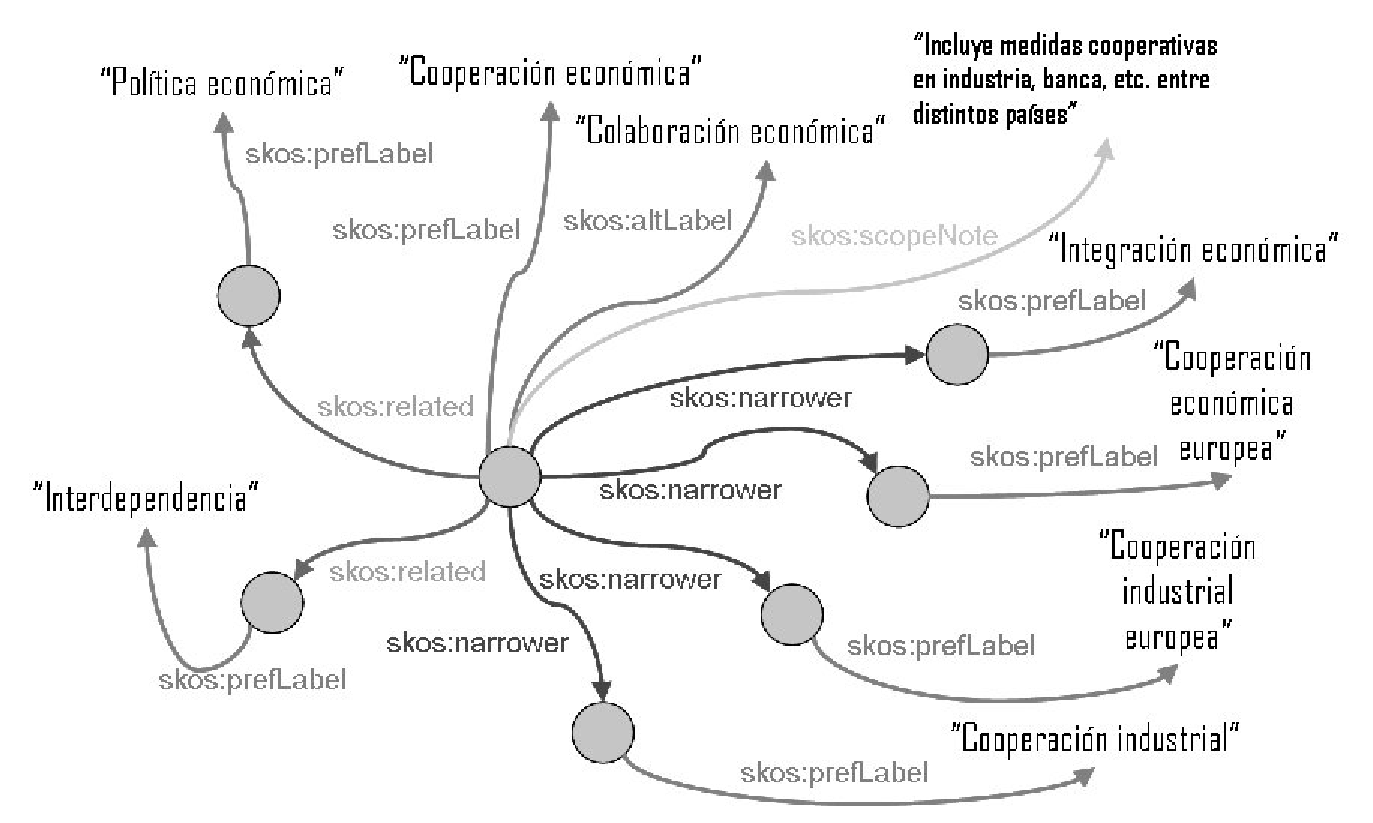
\includegraphics[width=14cm]{images/skos}
\caption{Concepto expresado en SKOS-Core.}
\label{fig:skos}
\end{figure}

Debe puntualizarse que el uso de SKOS-Core está siendo objeto de estudio para la
representación de recursos lexicográficos~\cite{Milin} desde un punto de vista de la
lingüística y como un avance tecnológico en este campo.

\item[\gls{FOAF} y \gls{DOAP}.] Vocabularios RDF para definir personas y amistades (\textit{Friend Of A Friend}), ver Figura~\ref{fig:foaf-example}, o 
proyectos (\textit{Description Of A Project}), 
ver Figura~\ref{fig:doap-example}. Cada vez hay un mayor interés por este tipo de tecnologías y algunos proyectos de gran envergadura como 
Apache o RDF Ohloh~\cite{Ferndez08rdfohloh}, que incluyen muchos subproyectos, programas, etc., utilizan estas
descripciones semánticas para cada módulo.

\begin{figure}[!htbp]
\centering
  \begin{lstlisting}
<#me> a foaf:Person;
	foaf:family_name "Alvarez Rodr\u00EDguez";
	foaf:givenname "Jose Mar\u00EDa";
	foaf:homepage <http://josemalvarez.es>;
	foaf:knows _:bnode2016979200;
	foaf:mbox_sha1sum "0d1d9ad2de64fd900d03c18e3d2608171832d155";
	foaf:name "Jose Mar\u00EDa Alvarez Rodr\u00EDguez";
	foaf:nick "chema";
	foaf:phone <tel:+34-666-714-721>;
	foaf:schoolHomepage <http://www.uniovi.es/inicio/>;
	foaf:title "Sr.";
	foaf:workplaceHomepage <http://www.weso.es>.
_:bnode2016979200 a foaf:Person;
	rdfs:seeAlso <http://www.di.uniovi.es/~labra/labraFoaf.rdf>;
	foaf:mbox_sha1sum "5fa5d69bac0c1396825c475ec19325ec0ffd5569";
	foaf:name "Jose Emilio Labra".
  \end{lstlisting}
\caption{Ejemplo parcial de documento FOAF en N3.}
\label{fig:foaf-example}
\end{figure}


\begin{figure}[!htbp]
\centering
  \begin{lstlisting}
<http://rdfohloh.wikier.org/project/moldeas/rdf> 
	dct:isFormatOf 	<http://rdfohloh.wikier.org/project/moldeas>;
	a foaf:Document;
	rdfs:label "MOLDEAS's DOAP document serialized in RDF/XML";
	foaf:primaryTopic <http://rdfohloh.wikier.org/project/moldeas>.
	<http://rdfohloh.wikier.org/project/moldeas> dct:updated "2012-01-22T13:02:25Z";
	rdfohloh:ohloh-page <http://www.ohloh.net/projects/moldeas>;
	doap:created "2011-10-14T09:19:11Z";
	doap:description "This work aims to apply the semantic web and 
	    LOD approaches to public procurement notices...";
	doap:download-page <http://code.google.com/p/moldeas/downloads/list>;
	doap:homepage <http://purl.org/weso/moldeas/>;
	doap:name "MOLDEAS";
	doap:programming-language "JavaScript";
	a doap:Project;
	= <http://rdfohloh.wikier.org/project/586667>;
	skos:subject <http://dbpedia.org/resource/Java>, 
	<http://dbpedia.org/resource/JavaScript>.
  \end{lstlisting}
\caption{Ejemplo parcial de documento DOAP en N3.}
\label{fig:doap-example}
\end{figure}

\item[\gls{SIOC}.] (\textit{Semantically-Interlinked Online Communities}). Es una ontología desarrollada 
por el equipo de Web Semántica de DERI Galway para describir semánticamente
distintas comunidades \textit{online}. SIOC integra, ver Figuras~\ref{fig:sioc} y~\ref{fig:sioc-example}, distintos vocabularios RDF con el
objetivo de reutilizar las definiciones ya realizadas en \gls{FOAF}, \gls{SKOS},
\gls{RSS} o \textit{Dublin Core}. Se ha empleado con éxito en distintas aplicaciones para gestionar y
describir toda la información disponible de las comunidades \textit{online}: listas de correo (SWAML~\cite{Sergio}), 
foros, etc.
 
\begin{figure}[!htb]
\centering
	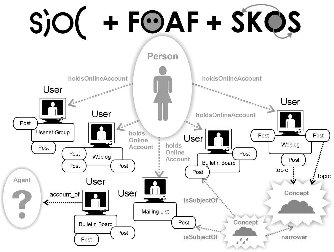
\includegraphics[width=12cm]{images/sioc}
\caption{SIOC integración con otros vocabularios.}
\label{fig:sioc}
\end{figure}

\begin{figure}[!htbp]
\centering
  \begin{lstlisting}
<rdf:RDF
  xmlns:sioc='http://rdfs.org/sioc/ns#'
  xmlns:rdf='http://www.w3.org/1999/02/22-rdf-syntax-ns#'
  xmlns:dc='http://purl.org/dc/elements/1.1/'
  xmlns:mvcb='http://webns.net/mvcb/'
>
  <sioc:Site rdf:about="http://groups.google.com/group/sioc-dev">
    <sioc:host_of>
      <sioc:Forum rdf:about="http://swaml.berlios.de/demos/sioc-dev/index.rdf#SIOC-Dev">
        <dc:description>SIOC development mailing list</dc:description>
        <mvcb:errorReportsTo rdf:resource="http://swaml.berlios.de/bugs"/>
        <sioc:container_of rdf:resource="http://swaml.berlios.de/demos/sioc-dev/2006-Dec/post-419.rdf"/>
        <dc:date>2007-06-18</dc:date>
        <dc:title>SIOC-Dev</dc:title>
        <mvcb:generatorAgent rdf:resource="http://swaml.berlios.de/doap.rdf"/>
        <sioc:has_host rdf:resource="http://groups.google.com/group/sioc-dev"/>
        <sioc:has_subscriber rdf:resource="http://swaml.berlios.de/demos/sioc-dev/subscribers.rdf#s26"/>
      </sioc:Forum>
    </sioc:host_of>
  </sioc:Site>
</rdf:RDF>
  \end{lstlisting}
\caption{Ejemplo de descripción con SIOC.}
\label{fig:sioc-example}
\end{figure}

\item[\gls{RSS}.] Existen diferentes versiones y definiciones de este vocabulario RDF, ver Figura~\ref{fig:rss-example}: \textit{Rich Site Summary} (RSS 0.91), XML; 
\textit{RDF Site Summary} (RSS 0.9 y 1.0), RDF; \textit{Really Simple Syndication} (RSS 2.0). La definición
realizada en el \gls{W3C} es la siguiente:

\begin{Frame}
Vocabulario RDF basado en XML que permite la catalogación de información (noticias y eventos) 
de los usuarios. Los archivos RSS contienen metadatos sobre fuentes de información especificadas 
por los usuarios, cuya función principal es notificar de forma automática cualquier cambio que se realice 
en esos recursos de interés.
\end{Frame}

\begin{figure}[!htb]
\centering
\lstinputlisting[language=XML]{examples/rss.rss}
\label{fig:rss-example}
\caption{Ejemplo de canal RSS.}
\end{figure}

\end{description}

En resumen, se dispone de un lenguaje muy útil y sencillo para describir recursos (RDF) y 
un esfuerzo en forma de vocabulario para la definición de recursos más detallada (RDFS) pero incompleto. 
Por ello, a continuación, se expondrán algunos de los lenguajes más completos que han surgido para 
intentar mejorar los puntos débiles de esta primera aproximación para la expresión de modelos semánticos. En cuanto
a vocabularios RDF existen una infinidad~\cite{common-vocabularies} de ellos para ser utilizados en distintos contextos que han sido
enormemente impulsados por la corriente \linkeddata y \opendata.
%Avoiding too many floats 
\clearpage

\subsubsection{OIL}
El \textit{Ontology Inference Layer}~\cite{Fensel01oil:an} (\gls{OIL}) desarrollado en el proyecto Europeo 
\textit{OntoKnowledge} está construido por encima de \gls{RDF} y RDFS utilizando muchos de sus constructores e intentando
mantener la compatibilidad hacia atrás. OIL provee características de modelado
basada en lógica de marcos~\cite{Kifer:1989:FHL:66926.66939} y \textit{Description Logic}~\cite{baader03description}.

La importancia de OIL reside en la unificación de:
\begin{itemize}
\item \textit{Description Logic}, heredando su semántica formal y la capacidad
de razonamiento efectivo (FaCT++, Racer o Pellet).
\item Sistemas basados en marcos, incorpora las características básicas de
modelado basado en marcos (conceptos, superclases, atributos, etc.).
\item Estándares web, construido sobre RDF y RDFS y utilizando como formato de
intercambio de datos XML.
\end{itemize}

Las ontologías creadas con OIL distinguen distintos meta niveles, con el
objetivo de proporcionar distintos niveles de servicio que pueden ser válidos para un
gran número de ontologías y aplicaciones:
\begin{description}
\item[Primer meta nivel:] también conocido como \textit{definición de ontologías}, en la
cual se proveen las definiciones de ontología, terminología que debería ser
instanciada para definir un vocabulario estructurado con la semántica adecuada.
\item[Segundo meta nivel:] conocido como ``meta meta'' nivel o \textit{contenedor de
ontologías}, describe las características de la ontología tales como autor,
nombre, ámbito, etc. Las anotaciones de este nivel se hacen mediante
\textit{Dublin Core}.
\end{description}

La capacidad de razonamiento es otra de las características importantes de OIL, que no estaba presente en RDF. Habitualmente esta capacidad se utiliza
para realizar las operaciones de clasificación, validación de consistencia e inferencia de nuevo conocimiento de acuerdo a distintos 
niveles de expresividad: 

\begin{description}
\item[Core OIL:] prácticamente compatible con RDFS exceptuando la capacidad de
``reificación''.
\item[Standard OIL:] lenguaje que captura las primitivas y constructores necesarios para
construir modelos semánticos con capacidad de inferencia.
\item[Instance OIL:] inclusión de ``instancias''.
\item[Heavy OIL:] capacidades extras de representación y razonamiento.
\end{description}


\begin{figure}[htb]
\centering
	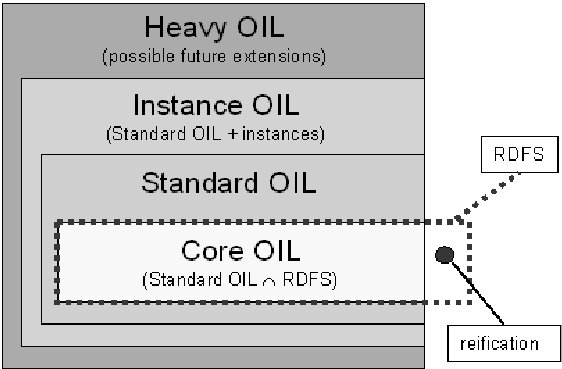
\includegraphics[width=10cm]{images/oil}
\caption{Niveles de expresividad OIL.}
\label{fig:oil}
\end{figure}

Cabe concluir, por tanto, que las principales ventajas de OIL se resumen en:
\begin{inparaenum} \item una aplicación no está obligada a trabajar con un
lenguaje más expresivo de lo necesario. \item aplicaciones que utilicen la
expresividad más baja pueden añadir aspectos de otras ontologías.
\item aplicaciones con un alto nivel de complejidad pueden utilizar
características de otras más simples.\end{inparaenum}

El trabajo realizado en OIL tiene su continuación en el siguiente lenguaje de
modelado de ontologías \gls{DAML+OIL}, ver Figura~\ref{daml+oil}, realizado por la cooperación
de iniciativas europeas y americanas.

\subsubsection{DAML+OIL}\label{daml+oil}
\gls{DAML+OIL}~\cite{HM00} es un lenguaje de marcado semántico para recursos web creado por la cooperación de las iniciativas
europeas (OIL) y americanas (DAML-ONT, \gls{DARPA} \textit{Agent Markup Language})
en el desarrollo de ontologías. El objetivo de desarrollo de este lenguaje está
especialmente centrado para la Web Semántica, modelización de dominios concretos,
utilizando los estándares (\gls{XML} y \gls{RDF}) y añadiendo una serie de primitivas de
orientación a objetos (clases, propiedades, axiomas y aserciones),
sistemas basados en marcos y parte de \textit{Description Logic}. Además, 
DAML+OIL da soporte a los tipos de datos de \gls{XML Schema}, separando las instancias
de una clase y de las instancias de tipos de datos. El significado de DAML+OIL
está definido por un modelo semántico estándar basado en las interpretaciones, consistiendo éstas 
en un dominio del discurso y una función de interpretación.

\subsubsection{OWL}\label{owl}
\gls{OWL}, lenguaje de ontologías para la web, sucesor de DAML+OIL, actualmente está
siendo desarrollado por el W3C, su primera versión estable es OWL 1.0, 
aunque que ya se ha publicado una nueva versión OWL 1.1~\cite{OWL11} y OWL2~\cite{owl2-primer}.

Como lenguaje para ontologías es una potente herramienta que dota de la
expresividad necesaria para mejorar algunos de los servicios más utilizados en
la red de Internet: búsqueda, manejo del conocimiento, interacción entre agentes
automáticos etc. Desde un punto de vista más formal, OWL está formado por
un conjunto de primitivas o constructores de metamodelado que son el punto de
partida para operaciones más complejas, como las de razonamiento. Actualmente,
aunque las características genéricas de OWL tienen su origen en OIL, se distinguen
al menos 3 versiones de OWL (en su versión 1.0 y 1.1) dependiendo de su expresividad, complejidad y grado
de computabilidad, cada versión superior de OWL contiene a la anterior
($Lite\subset DL \subset FULL$).

\begin{description}
\item[OWL-FULL.] Se pueden utilizar todos los constructores y primitivas
definidos en OWL y no restringe el uso de RDF. Esto implica que no se garantiza
su decidibilidad pero en cambio, como familia de \textit{Description Logics}
posee un gran poder expresivo: tratar clases como instancias, definir
propiedades sobre tipos de datos (\textit{string}, \textit{float}, etc.) .

\item[OWL-DL.] Subconjunto decidible de OWL-FULL, supone la máxima expresividad
computable. Cada modelo realizado en OWL-DL genera directamente un modelo
semántico en \textit{Description Logics}.

\item[OWL-Lite.] Añade restricciones adicionales sobre en el uso de los
constructores de OWL, básicamente se pueden modelar jerarquías con restricciones
sencillas.
\end{description}

Para advertir a que nivel de expresividad y complejidad se puede trabajar
dependiendo del lenguaje utilizado se dispone la Figura~\ref{fig:owl-dialects}, extraída del laboratorio OntoText.

\begin{figure}[htb]
\centering
	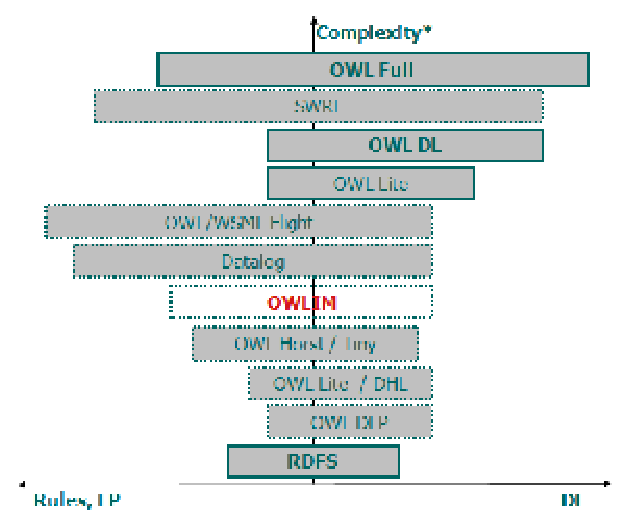
\includegraphics[width=10cm]{images/owl-dialects}
\caption{Algunos lenguajes para la Web Semántica por OntoText.}
\label{fig:owl-dialects}
\end{figure}


Algunas de las características que hacen interesante el uso de OWL en el ámbito
de la Web Semántica son:
\begin{itemize}
  \item Las ontologías en OWL son una serie de axiomas y hechos que pueden
  reutilizar otras ontologías (importándolas). Además, como documento que son
  (serializado en RDF/XML), están identificadas por un URI y tienen asociada cierta metainformación
  (author, dominio, fecha, etc.) que permite que sean referenciables como
  cualquier otro recurso en la red.
  \item Los axiomas son utilizados para asociar una serie de características
  (descripciones, restricciones, etc.) a las clases y propiedades de la
  ontología. 
\item Los hechos proporcionan información particular de una determinada instancia. 
\end{itemize}

Como ejemplo de utilización de OWL, en su versión DL y con características de OWL2, se presenta una sencilla
ontología, ver Figura~\ref{fig:psydiag}, que modela un sistema de diagnóstico psicológico con capacidad de clasificar individuos
de acuerdo a sus síntomas, ver Figura~\ref{fig:psydiag-axiomas}, con sintaxis Manchester.

\begin{figure}[htb]
\centering
	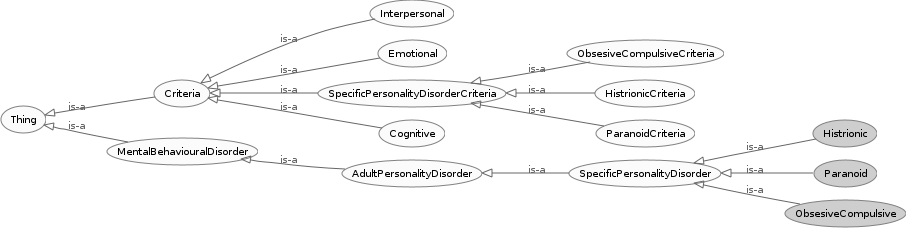
\includegraphics[width=16cm]{images/psydiag}
\caption{Ontología de ejemplo en OWL2 para diagnóstico psicológico.}
\label{fig:psydiag}
\end{figure}


\begin{figure}[htb]
\centering
 \begin{lstlisting} 
Class: <http://example.org/psydiag.owl/Histrionic>

    EquivalentTo: 
        <http://example.org/psydiag.owl/has-criteria> min 3
	      <http://example.org/psydiag.owl/HistrionicCriteria>,
        (not (<http://example.org/psydiag.owl/has-criteria> some 
	      <http://example.org/psydiag.owl/ObsesiveCompulsiveCriteria>))
         and (not (<http://example.org/psydiag.owl/has-criteria> some 
	      <http://example.org/psydiag.owl/ParanoidCriteria>))
         and (<http://example.org/psydiag.owl/has-criteria> only 
	      <http://example.org/psydiag.owl/HistrionicCriteria>)
    
    SubClassOf: 
        <http://example.org/psydiag.owl/SpecificPersonalityDisorder>

DisjointClasses: 
    <http://example.org/psydiag.owl/Histrionic>,
    <http://example.org/psydiag.owl/ObsesiveCompulsive>,
    <http://example.org/psydiag.owl/Paranoid>
  \end{lstlisting} 
\caption{Algunos axiomas de ejemplo en OWL2 para diagnóstico psicológico.}
\label{fig:psydiag-axiomas}
\end{figure}


\subsubsection{WSML}
\gls{WSML}~\cite{WSML2006} es la propuesta de lenguajes formales realizado en \gls{WSMO}~\cite{WSMODeri} 
(relevante por su relación con los Servicios Web Semánticos) para la construcción de ontologías y que recoge 
distintas variantes de lógica, ver Figura~\ref{fig:wsml-layering}. En general, teniendo en cuenta los
distintos tipos de lógica de acuerdo a su expresividad es posible obtener diferentes serializaciones
de los modelos realizados con distintos lenguajes \gls{OWL}, WSML, F-Logic, etc. Esta característica
es muy interesante para el uso de razonadores con distintos tipos de algoritmos y capacidades de
razonamiento, independientemente del lenguaje en el que se haya modelado el dominio.

\begin{figure}[htb]
\centering
	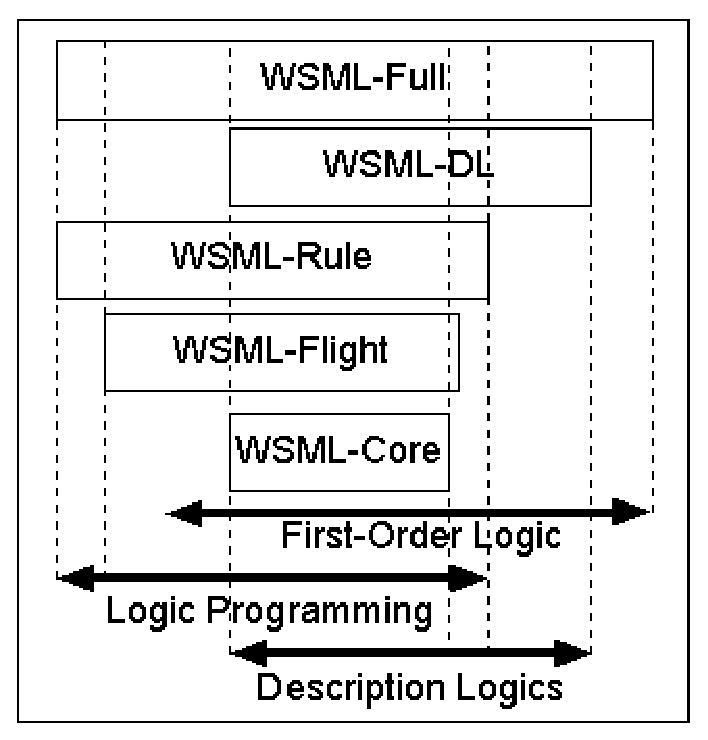
\includegraphics[width=8cm]{images/wsml-layering}
\caption{Capas de WSML.}
\label{fig:wsml-layering}
\end{figure}

\begin{note}
En OWL, con la arquitectura semántica de una torre, ver Figura~\ref{fig:stack-2002}, las
reglas ocuparían una capa por encima del lenguaje. Sin embargo, la práctica ha demostrado que la reglas son
parte de la ontología (no son condición necesaria, pero a un mínimo de complejidad en el
modelo se aprecia su utilidad). WSML incluye una variedad cubriendo esta
posibilidad (WSML-RULE).
\end{note}


\subsubsection{Nota}
Los lenguajes aquí presentados no son los únicos para la expresión de modelos de
conocimiento basados en semántica y reaprovechables para la web. No obstante,
al estar impulsados por el \gls{W3C} y pretender ser estándares, resultan de especial
interés y casi de conocimiento obligado para la comunidad de la Web Semántica.

No se puede determinar cuál es mejor que otro, la decisión de un lenguaje u otro
 debería venir asociado a un profundo análisis tanto funcional: propiedades  del
dominio a modelar y las necesidades lógicas del mismo como no funcional:
herramientas desarrollados, soporte, estabilidad, etc. Actualmente, \gls{OWL} 1.0
en su versión DL, \gls{WSML} y \gls{RDF} están siendo ampliamente utilizados mientras que las
propuestas de \gls{OIL}, \gls{DAML+OIL} y RDFS o bien están obsoletas o no han cumplido
las expectativas de los desarrolladores.


 
